\documentclass{report}
\usepackage[utf8]{inputenc}
\usepackage[slovene]{babel}
\usepackage{makeidx}
\usepackage{hyperref}
\usepackage{booktabs}
\usepackage{textgreek}
\usepackage{multirow} % for spanning rows
\usepackage{changepage}
\usepackage{ulem}
\usepackage{afterpage}
\usepackage{float}
\usepackage{bm}
\usepackage{mathtools}
\usepackage{amsmath}
\usepackage{graphicx}
\usepackage{pgfplots}
\usepackage{enumitem}
\graphicspath{ {./images/} }

\hypersetup{
  colorlinks=true,         % Colored links instead of boxes
  linkcolor=blue,          % Color for internal links
  citecolor=green,         % Color for citations
  filecolor=magenta,       % Color for file links
  urlcolor=cyan,           % Color for external links
  bookmarksopen=true,      % Display bookmarks when the PDF is opened
  bookmarksnumbered=true,  % Display section numbers in bookmarks
  bookmarksdepth=2,        % Set the depth of bookmarks (1 for chapters, 2 for sections, etc.)
}

\title{Vaje iz mehanike}
\author{Matija Zanjkovič\thanks{Mentor: Marko Šterk}}
\date{Maribor, 2023}

\begin{document}

\maketitle
\thispagestyle{empty}

\null\newpage

\thispagestyle{empty}
\tableofcontents

\listoftables

\listoffigures

\thispagestyle{empty}

\clearpage  % Start a new page



\setcounter{page}{1}  % Set the page number to 1

\chapter{Vaja 1: Merjenje gostote}
\section{Gostota trdne snovi}
\subsection{Naloga 1}
Z merjenjem dimenzij (širine (\bm{a}), višine (\bm{b}), dolžine (\bm{c})) in mase (\bm{m}) kvadra določite gostoto \bm{(\rho)} snovi, iz katere je narejen kvader. 
Gostoto izračunajte po enačbi \bm{\rho\ =\ m/V}, kjer je \bm{V} prostornina (\bm{V\ =\ abc}). Določite tudi napako gostote snovi.
\subsection{Sistematične napake merilnikov}
Napaka kljunastega merila: \bm{0.05\ mm}\\
Napaka mikrometra: \bm{0.01\ mm}\\
Napaka tehtnice: \bm{0.1\ g}\\

\subsection{Meritve}

% Tabela za meritev a
\begin{table}[H]
  \centering
  \caption{Meritve dimenzije a}
  \begin{adjustwidth}{-2 cm}{0 cm}
  \begin{tabular}{cccccccc}
  \toprule
  Meritev & $a_{izm}\ [mm]$ & $\overline{a}\ [mm]$ & $a_{izm} - \overline{a}\ [mm]$ & $\Delta a_{sist}\ [mm]$ & $\sigma [mm]$&  $\Delta a_{sl}\ [mm]$ & $a\ [mm]$\\
  \midrule
  1 & 8.16 & \multirow{10}{*}{8.16} & 0 & \multirow{10}{*}{0.01} & \multirow{10}{*}{0.02} & \multirow{10}{*}{0.01} \\
  2 & 8.15 &  & -0.01 &\\
  3 & 8.20 &  & \sout{0.04} &\\
  4 & 8.18 &  & 0.02 &\\
  5 & 8.16 &  & 0.00 & & & & 8.16 \ \pm \ 0.02\\
  6 & 8.15 &  & -0.01 & & & & = \\
  7 & 8.16 &  & 0.00 & & & & 8.16 $\cdot$ (1 \ \pm \ 0.002)\\
  8 & 8.17 &  & 0.01 &\\
  9 & 8.10 &  & \sout{-0.06} &\\
  10 & 8.12 &  & \sout{-0.04} &\\
  % Add more rows here
  \bottomrule
  \end{tabular}
  \end{adjustwidth}
\end{table}

% Tabela za meritev b
\begin{table}[H]
  \centering
  \caption{Meritve dimenzije b}
  \begin{adjustwidth}{-2 cm}{0 cm}
  \begin{tabular}{cccccccc}
  \toprule
  Meritev & $b_{izm}\ [mm]$ & $\overline{b}\ [mm]$ & $b_{izm} - \overline{b}\ [mm]$ & $\Delta b_{sist}\ [mm]$ & $\sigma\ [mm]$ & $\Delta b_{sl}\ [mm]$ &  $b\ [mm]$\\
  \midrule
  1 & 25.25 & \multirow{10}{*}{25.23} & 0.02 & \multirow{10}{*}{0.05} & \multirow{10}{*}{0.03} & \multirow{10}{*}{0.01}\\
  2 & 25.20 &  & -0.03 &\\
  3 & 25.20 &  & -0.03 &\\
  4 & 25.25 &  & 0.02 &\\
  5 & 25.25 &  & 0.02 & & & & 25.23 \ \pm \ 0.06\\
  6 & 25.20 &  & \sout{-0.03} & & & & =\\
  7 & 25.20 &  & \sout{-0.03} & & & & 25.23 $\cdot$ (1 \ \pm \ 0.002)\\
  8 & 25.20 &  & \sout{-0.03} &\\
  9 & 25.25 &  & 0.02 &\\
  10 & 25.25 &  & 0.02 &\\
  % Add more rows here
  \bottomrule
  \end{tabular}
  \end{adjustwidth}
\end{table}

% Tabela za meritev c
\begin{table}[H]
  \centering
  \caption{Meritve dimenzije c}
  \begin{adjustwidth}{-2 cm}{0 cm}
  \begin{tabular}{cccccccc}
  \toprule
  Meritev & $c_{izm}\ [mm]$ & $\overline{c}\ [mm]$ & $c_{izm} - \overline{c}\ [mm]$ & $\Delta c_{sist}\ [mm]$ & \sigma & $\Delta c_{sl}\ [mm]$ & $c\ [mm]$\\
  \midrule
  1 & 40.00 & \multirow{10}{*}{40.02} & -0.02 & \multirow{10}{*}{0.05} & \multirow{10}{*}{0.02} & \multirow{10}{*}{0.01} & \multirow[b]{4}{*}{40.02 \ \pm \ 0.06}\\
  2 & 40.00 &  & -0.02 &\\
  3 & 40.10 &  & \sout{0.08} &\\
  4 & 40.00 &  & -0.02 &\\
  5 & 40.00 &  & -0.02 & & & & \multirow{2}{*}{=}\\
  6 & 40.00 &  & -0.02 & & &  \\
  7 & 40.00 &  & -0.02 & & & & \multirow[t]{4}{*}{40.02 $\cdot$ (1 \ \pm \ 0.001)} \\
  8 & 40.05 &  & \sout{0.03} &\\
  9 & 40.05 &  & \sout{0.03} &\\
  10 & 40.00 &  & -0.02 &\\
  % Add more rows here
  \bottomrule
  \end{tabular}
  \end{adjustwidth}
\end{table}

Meritev mase: $m = 22.8 \ \pm \ 0.1\ g \ = \ 22.8 \cdot (1 \ \pm \ 0.004)\ g$

\pagebreak

\subsection{Računanje gostote}

Gostota se računa po enačbi:
\begin{equation}
  \rho = \frac{m}{V}
\end{equation}
\\
Vendar najprej rabimo volumen telesa. Ker gre za kvader lahko uporabimo enačbo:
\begin{equation}
  V = abc
\end{equation}
\\
Tako torej dobimo:

\begin{equation}
  \label{eq:1}
  \begin{gathered}
    V = 8.16 \ (1 \pm 0.002)\ mm \cdot 25.23 \ (1 \pm 0.002)\ mm \cdot 40.02 \ (1 \pm 0.001)\ mm\\
    V = 8.16 \cdot 25.23 \cdot 40.02 \ (1 \pm (0.002 + 0.002 + 0.001))\ mm^3\\
    V = 8240 \ (1 \pm 0.005) \ mm^3
  \end{gathered}
\end{equation}
\\
Sedaj lahko izračunamo gostoto telesa:

\begin{equation}
  \label{eq:1}
  \begin{gathered}
    \rho = \frac{22.8 \cdot (1 \ \pm \ 0.004)\ g}{8240 \cdot (1 \pm 0.005) \ mm^3} \\
    \rho = 2.77 \cdot 10^{-3} \cdot (1 \ \pm \ 0.009) \ \frac{g}{mm^3} \\
    \rho = 2.77 \cdot 10^3 \cdot (1 \ \pm \ 0.009) \ \frac{kg}{m^3}
  \end{gathered}
\end{equation}

\subsection{Rezultati}
Prišli smo do rezultata, da je gostota telesa $\rho = 2770 \cdot (1 \ \pm \ 0.009) \ \frac{kg}{m^3}$ oz. 
$\rho = (2,77 \ \pm \ 0.02) \cdot 10^3 \ \frac{kg}{m^3}$.
\\\\
S tega bi lahko sklepali, da je telo verjetno iz zlitine, ki vsebuje veliko aluminija, saj je njegova gostota: 
$\rho_{Al} = 2710 \ \frac{kg}{m^3}$.


\pagebreak

\section{Gostota kapljevine}
\subsection{Naloga 2}
\textbf{a)} Z menzuro in tehtnico izmerite gostoto 20 \% raztopine kuhinjske soli v vodi. Gostoto izmerite tudi z areometrom.\\\\
\textbf{b)} Z areometrom izmerite gostoto etilnega alkohola.

\subsection{Sistematične napake merilnikov}
Napaka areometra za raztopino NaCl: $\bm{0.01 \ \left[ \frac{g}{mL} \right]}$ \\
Napaka areometra za etilni alkohol: $\bm{0.005 \ \left[ \frac{g}{mL} \right]}$ \\
Merilno območje termometra: od $\bm{-199.9\ ^{\circ}C$} do \bm{$199.9\ ^{\circ}C}$ \\
Napaka tehtnice: \bm{1\ g} \\
Napaka menzure: \bm{2\ mL}
\\

\pagebreak

\subsection{Postopek in meritve}

Najprej smo pripravili 20 \% raztopino NaCl. Skupna masa raztopine je bila:
\begin{equation}
  m = (620 \ \pm \ 1 )\ g 
\end{equation}
\\
Nato smo izmerili volumen naše raztopine. Ker je menzura bila premajhna za 
celotno meritev volumna, smo to morali narediti trikrat.

\begin{equation}
  \label{eq:1}
  \begin{gathered}
    V = (250 \ mL \ \pm \ 2 \ mL) \ + \ (250 \ mL \ \pm \ 2 \ mL) + (51 \ mL \ \pm \ 2 \ mL) \\
    V = (553 \ \pm \ 6) \ mL \\
    V = 553 \cdot (1 \ \pm \ 0.01) \ mL
  \end{gathered}
\end{equation}
\\

Nato smo gostoto raztopine NaCl izmerili še z areometrom.

% Tabela za meritev gostote raztopine NaCl
\begin{table}[H]
  \centering
  \caption{Meritve gostote raztopine NaCl z areometrom}
  \begin{adjustwidth}{-2cm}{0cm}
  \begin{tabular}{cccccccc}
  \toprule
  Meritev & $\rho_{izm} \left[ \frac{g}{mL} \right]$ & $\overline{\rho}\ \left[ \frac{g}{mL} \right]$ & $\rho_{izm} - \overline{\rho}\ \left[ \frac{g}{mL} \right]$ & $\Delta \rho_{sist}\ \left[ \frac{g}{mL} \right]$ & $\Delta \rho_{sl}\ \left[ \frac{g}{mL} \right]$ & $\rho\ \left[ \frac{g}{mL} \right]$ & $T \ [^{\circ}C] $\\
  \midrule
  1 & 1.14 & \multirow{5}{*}{1.14} & 0 & \multirow{5}{*}{0.01} & \multirow{5}{*}{0} & & \multirow{5}{*}{19.6}\\
  2 & 1.14 &  & 0 & & & $1.14 \ \pm \ 0.01 $\\
  3 & 1.15 &  & \sout{0.01} & & & = \\
  4 & 1.14 &  & 0 & & & $1.14 \cdot (1 \ \pm \ 0.01)$\\
  5 & 1.15 &  & \sout{0.01} & & & \\
  % Add more rows here
  \bottomrule
  \end{tabular}
  \end{adjustwidth}
\end{table}

Nato smo še opravili meritve gostote etilnega alkohola, s pomočjo areometra.

\begin{table}[H]
  \centering
  \caption{Meritve gostote etilnega alkohola}
  \begin{adjustwidth}{-2cm}{0cm}
  \begin{tabular}{cccccccc}
  \toprule
  Meritev & $\rho_{izm} \left[ \frac{g}{mL} \right]$ & $\overline{\rho}\ \left[ \frac{g}{mL} \right]$ & $\rho_{izm} - \overline{\rho}\ \left[ \frac{g}{mL} \right]$ & $\Delta \rho_{sist}\ \left[ \frac{g}{mL} \right]$ & $\Delta \rho_{sl}\ \left[ \frac{g}{mL} \right]$ & $\rho\ \left[ \frac{g}{mL} \right]$ & $T \ [^{\circ}C] $\\
  \midrule
  1 & 0.805 & \multirow{5}{*}{0.805} & 0 & \multirow{5}{*}{0.005} & \multirow{5}{*}{0} & & \multirow{5}{*}{21.5} \\
  2 & 0.805 &  & 0 & & & 0.805 \ \pm \ 0.005 \\
  3 & 0.805 &  & 0 & & & = \\
  4 & 0.805 &  & 0 & & & 0.805 \cdot (1 \ \pm \ 0.006)\\
  5 & 0.805 &  & 0 & & & \\
  % Add more rows here
  \bottomrule
  \end{tabular}
  \end{adjustwidth}
\end{table}

\pagebreak

\subsection{Računanje gostote}

Računanje gostote 20 \% raztopine NaCl s pomočjo mase in volumna:

\begin{equation}
  \label{eq:1}
  \begin{gathered}
    \rho = \frac{620 \cdot (1 \ \pm \ 0.002)\ g}{553 \cdot (1 \pm 0.01) \ mL} \\
    \rho = 1.12 \cdot (1 \ \pm \ 0.01) \ \frac{g}{mL} \\
    \rho = 1120 \cdot (1 \ \pm \ 0.01) \ \frac{kg}{m^3}
  \end{gathered}
\end{equation}

\subsection{Rezultati}

Prišli smo do rezultatov, da je gostota NaCl pridobljena s tehtananjem in merjenjem dimenzij: 
$ \rho_{NaCl} = 1120 \cdot (1 \ \pm \ 0.01) \ \frac{kg}{m^3} $ oz. $ \rho_{NaCl} = (1120 \ \pm \ 10) \ \frac{kg}{m^3} $.
 Meritev z areometrom pa: $ \rho_{NaCl} = 1140 \cdot (1 \ \pm \ 0.01) \ \frac{kg}{m^3}$ oz. 
 $ \rho_{NaCl} = (1140 \ \pm \ 10) \ \frac{kg}{m^3} $. Do odstopanja pri različnih metodah je mogoče prišlo, 
 zaradi nenatančnosti pri merjenju, ali pa se je mogoče temperatura raztopine malo spremenila.

\medskip

\noindent Gostoto etilnega alkohola pa sem izmeril samo z areometrom in dobil: 
$ \rho_{alkohol} = 805 \cdot (1 \ \pm \ 0.006) \ \frac{kg}{m^3} $ oz. $ \rho_{alkohol} = (805 \ \pm \ 5) \ \frac{kg}{m^3} $


\pagebreak
\section{Vprašanja}
\textbf{a)} Razložite, kako temperatura vpliva na merjenje gostote 
kapljevine. Za koliko odstotkov se spremeni gostota vode, če se 
temperatura spremeni za \bm{$1 \ K$}? Temperaturni koeficient prostorninskega 
razteska vode je \bm{$2.06 \cdot 10^{-6}K^{-1}$.}
\\\\
Relativno povečanje volumna vode je sorazmerno spremembi temperature:
\begin{equation}
  \frac{\Delta V}{V} = \beta \Delta T
\end{equation}
Če torej v enačbo vstavimo podatke dobimo:
\begin{equation}
  \label{eq:1}
  \begin{gathered}
    \frac{\Delta V}{V} = 2.06 \cdot 10^{-6}K^{-1} \cdot 1 \ K \\
    \frac{\Delta V}{V} = 2.06 \cdot 10^{-4} \%
  \end{gathered}
\end{equation}
\\

\noindent Torej bi se voda razteznila za $2.06 \cdot 10^{-4} \%$.

\bigskip


\noindent
\textbf{b)} Razložite fizikalni princip meritve gostote tekočin z areometrom. \\

\noindent
Areometer deluje na podlagi vzgona tekočine, v katero je potopljen.
Ima obliko ozke cevi z utežjo na dnu, ki je dovolj težka, da se areometer potopi v tekočino. 
Ko je areometer potopljen v tekočino, se potopi do ravni, kjer je vzgon enak teži areometra. 
Ta raven potopljenosti je odvisna od gostote tekočine.

\chapter{Vaja 2: Merjenje sile}

\section{Naloga}

\textbf{a)} Izvedite eksperiment, pri katerem boste merili silo v vzmeti in raztezek vzmeti. 
Izmerjene podatke prikažite z odvisnostjo sile vzmeti od raztezka. 
Iz diagrama določite prožnostni koeficient vzmeti.
\\\\
\textbf{b)} Sestavite vzmetno nihalo in izmerite silo v vzmeti v odvisnosti od časa. 
Meritev izvedite z računalniškim merilnim sistemom Vernier. 
Meritev opravite s tremi različnimi utežmi. 
Iz diagrama sile v odvisnosti od časa v vseh treh primerih odčitajte nihajni čas nihala in v vsakem primeru izračunajte konstanto vzmeti.

\section{Sistematične napake merilnikov}

Napaka ravnila: $\bm{0.1 \ cm}$ \\
Napaka tehtnice: $\bm{0.1 \ g}$ \\
Napaka za čas: $\frac{0.01}{15} \ s = \bm{0.001 \ s}$

\pagebreak

\section{Merjenje}

Za določanje koeficienta vzmeti sem najprej izmeril raztezke pri različnih masah uteži.

\begin{table}[H]
  \label{table:F(x)}
  \centering
  \caption{Raztezek vzmeti pri določeni teži}
  \begin{adjustwidth}{0cm}{0cm}
  \begin{tabular}{ccccccccc}
  \toprule
  Meritev & $m \ [g]$ & $\Delta m \ [g]$ & $ F \ [N] $ & $\Delta F \ [N]$ & $ x \ [cm] $ & $\Delta \ x \ [cm]$  \\
  \midrule
  1 & 50.9 & \multirow{7}{*}{0.1} & 0.499 & \multirow{7}{*}{0.001} & 6.8 & \multirow{7}{*}{0.1} & \\
  2 & 100.9 &  & 0.990 & & 13.5 & \\
  3 & 148.9 &  & 1.461 & & 19.8 &  \\
  4 & 199.4 &  & 1.956 & & 26.6 & \\
  5 & 148.9 &  & 1.461 & & 19.8 & \\
  6 & 100.9 &  & 0.990 & & 13.4 & \\
  7 & 50.9 &  & 0.499 & & 6.6 & \\
  % Add more rows here
  \bottomrule
  \end{tabular}
  \end{adjustwidth}
\end{table}

\noindent
Nato sem za uteži z masami $50.9  \ g$, $100.9 \ g$ in $148.9 \ g$ izmeril čas
nihanja za 15 nihajev.  


\begin{table}[H]
  \centering
  \caption{Nihajni čas}
  \begin{adjustwidth}{-3cm}{0cm}
  \begin{tabular}{cccccccccc}
  \toprule
  Meritev & $m \ [g]$ & $t_{izm} [s]$ & $t_{en \ nihaj} [s]$ &$ \overline{t} \ [s]$ & $t_{en \ nihaj} \ - \ \overline{t} \ [s]$ & $ \sigma \ [s] $ & $\Delta \ t_{sl} \ [s]$ & $ \Delta \ t_{sist} $ & $t \ [s]$\\
  \midrule
  1 & \multirow{5}{*}{50.9} & 8.26 & 0.551 & \multirow{5}{*}{0.551} & 0 & \multirow{5}{*}{0} & \multirow{5}{*}{0} & \multirow{5}{*}{0.001} &  \multirow{2}{*}{$0.551 \ \pm \ 0.001$}\\
  2 &  & 8.26 & 0.551 & & 0 & & & & \\
  3 &  & 8.24 & 0.549 & & \sout{-0.001} & & & & = \\
  4 &  & 8.26 & 0.551 & & 0 & & & & \multirow{2}{*}{$0.551 \cdot (1 \ \pm \ 0.002)$} \\
  5 &  & 8.28 & 0.552 & & \sout{0.001} & \\
  \midrule
  1 & \multirow{4}{*}{100.9} & 11.40 & 0.7600 & \multirow{5}{*}{0.7272} & \sout{0.0328} & \multirow{5}{*}{0.0219} & \multirow{5}{*}{0.0069} & \multirow{5}{*}{0.0007} & \multirow{2}{*}{$0.7272 \ \pm \ 0.014$}\\
  2 & & 10.58 & 0.7053 & & -0.0219 & & & & \\
  3 & & 10.60 & 0.7067 & & -0.0205 & & & & = \\
  4 & & 10.62 & 0.7080 & & -0.0192 & & & & \multirow{2}{*}{$0.7272 \cdot (1 \ \pm \ 0.02)$} \\
  5 & & 11.34 & 0.7560 & & \sout{0.0288}\\

  \midrule
  1 & \multirow{5}{*}{148.9} & 13.64 & 0.9093 & \multirow{5}{*}{0.9099} & -0.0006 & \multirow{5}{*}{0.0008} & \multirow{5}{*}{0.0004} & \multirow{5}{*}{0.0007} & \multirow{2}{*}{$0.9098 \ \pm \ 0.0008$}\\
  2 & & 13.64 & 0.9093 & & -0.0006 & & & & \\
  3 & & 13.66 & 0.9107 & & 0.0008 & & & & = \\
  4 & & 13.62 & 0.9080 & & \sout{-0.0019} & & & & \multirow{2}{*}{$0.9099 \cdot (1 \ \pm \ 0.0009)$}\\
  5 & & 13.68 & 0.9120 & & \sout{0.0021}\\
  % Add more rows here
  \bottomrule
  \end{tabular}
  \end{adjustwidth}
\end{table}

\pagebreak

\section{Rezultati}

\subsection{Prožnostni koeficient vzmeti}

Enačba za izračun raztezka je:

\begin{equation}
  F = kx
\end{equation}

\noindent Če izpostavimo prožnostni koeficient vzmeti dobimo:

\begin{equation}
  k = \frac{F}{x}
\end{equation}

\noindent S pomočjo podatko iz tabele 2.1, narišemo graf sile v odvisnosti od raztezka,
da dobimo graf F(x).
  


\begin{figure}[H]
  \caption{Graf F(x)}
  \label{fig:graf}
  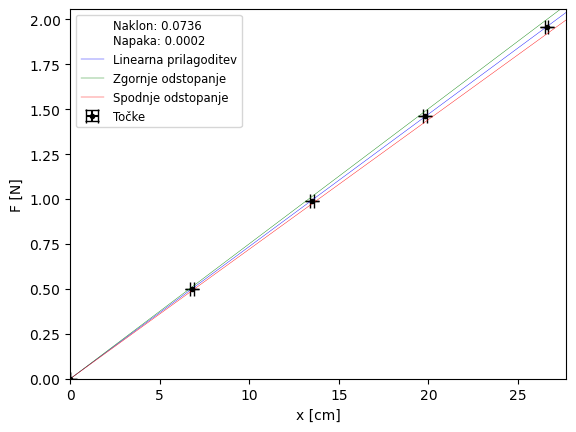
\includegraphics[width=\textwidth]{F(x)}
\end{figure}

Iz tega je razvidno, da je koeficient prožnosti vzmeti enak:

\begin{equation}
  k = (0.0736 \pm 0.0002) \ \frac{N}{cm}
\end{equation}

\pagebreak

\subsection{Izračun konstane vzmeti}

\noindent Pri tem delu naloge je za vsako izmed uteži treba izračunati konstanto vzmeti.
\\
\noindent Za vzmet, ki niha velja sledeča enačba:

\begin{equation}
  t_0 = 2 \pi \sqrt{\frac{m}{k}}
\end{equation}

\noindent Nas pri tem zanima, konstanto vzmeti.

\begin{equation}
  k = m \left(\frac{2 \pi}{t_0}\right)^2
\end{equation}

\noindent \underline{Izračun za prvo utež:}

\noindent $m_1 = 50.9 \cdot (1 \ \pm \ 0.002) \ g = 50.9 \cdot 10^{-3} \cdot (1 \ \pm \ 0.002) \ kg$ \\
$t_{0_1} = 0.551 \cdot (1 \ \pm \ 0.002) \ s$

\begin{equation}
  \label{eq:1}
  \begin{gathered}
    k_1 = 50.9 \cdot 10^{-3} \cdot (1 \ \pm \ 0.002) \ kg \cdot \left(\frac{2 \pi}{0.551 \cdot (1 \ \pm \ 0.002) \ s}\right)^2 \\
    k_1 = 50.9 \cdot 10^{-3} \cdot (1 \ \pm \ 0.002) \ kg \cdot \frac{4 {\pi}^2}{0.551^2 \cdot (1 \ \pm \ 2 \cdot 0.002) \ s^2} \\
    k_1 = \frac{50.9 \cdot 10^{-3} \cdot 4 {\pi}^2}{0.551^2} \cdot (1 \ \pm \ 0.004) \frac{kg}{s^2} \\
    \boxed {k_1 = 6.62 \cdot (1 \ \pm \ 0.004) \frac{N}{m}}
  \end{gathered}
\end{equation}


%%%%%%%%%%%%% Druga utež %%%%%%%%%%%%%%%%%%

\noindent \underline{Izračun za drugo utež:}

\noindent $m_2 = 100.9 \cdot (1 \ \pm \ 0.001) \ g = 100.9 \cdot 10^{-3} \cdot (1 \ \pm \ 0.001) \ kg$ \\
$t_{0_2} = 0.7272 \cdot (1 \ \pm \ 0.02) \ s$

\begin{equation}
  \label{eq:1}
  \begin{gathered}
    k_2 = 100.9 \cdot 10^{-3} \cdot (1 \ \pm \ 0.001) \ kg \cdot \left(\frac{2 \pi}{0.7272 \cdot (1 \ \pm \ 0.02) \ s}\right)^2 \\
    k_2 = 100.9 \cdot 10^{-3} \cdot (1 \ \pm \ 0.001) \ kg \cdot \frac{4 {\pi}^2}{0.7272^2 \cdot (1 \ \pm \ 2 \cdot 0.02) \ s^2} \\
    k_2 = \frac{100.9 \cdot 10^{-3} \cdot 4 {\pi}^2}{0.7272^2} \cdot (1 \ \pm \ 0.04) \frac{kg}{s^2} \\
    \boxed {k_2 = 7.533 \cdot (1 \ \pm \ 0.04) \frac{N}{m}}
  \end{gathered}
\end{equation}

\pagebreak
%%%%%%%%%%%%% Tretja utež %%%%%%%%%%%%%%%%%%

\noindent \underline{Izračun za tretjo utež:}

\noindent $m_2 = 148.9 \cdot (1 \ \pm \ 0.0007) \ g = 1048.9 \cdot 10^{-3} \cdot (1 \ \pm \ 0.0007) \ kg$ \\
$t_{0_2} = 0.9098 \cdot (1 \ \pm \ 0.0009) \ s$

\begin{equation}
  \label{eq:1}
  \begin{gathered}
    k_3 = 148.9 \cdot 10^{-3} \cdot (1 \ \pm \ 0.0007) \ kg \cdot \left(\frac{2 \pi}{0.9098 \cdot (1 \ \pm \ 0.0009) \ s}\right)^2 \\
    k_3 = 148.9 \cdot 10^{-3} \cdot (1 \ \pm \ 0.0007) \ kg \cdot \frac{4 {\pi}^2}{0.9098^2 \cdot (1 \ \pm \ 2 \cdot 0.0009) \ s^2} \\
    k_3 = \frac{148.9 \cdot 10^{-3} \cdot 4 {\pi}^2}{0.9098^2} \cdot (1 \ \pm \ 0.003) \frac{kg}{s^2} \\
    \boxed {k_3 = 7.102 \cdot (1 \ \pm \ 0.003) \frac{N}{m}}
  \end{gathered}
\end{equation}

\pagebreak

\section{Vprašanje}

\textbf{a)} Kaj si predstavljate pod električnim uporom materiala in zakaj se ta spreminja, ko material izpostavimo električnemu toku?
\\\\
\noindent
Pod \textit{električnim uporom} materiala si predstavljam, kako močno material ovira pretok električnega toka pri določeni napetosti. Večji kot je upor, manj toka bo teklo skozi material.

\textbf{Dejavniki, ki vplivajo na upornost materiala:}
\begin{itemize}
    \item \textbf{Tip materiala:} Snovi z več prostimi nosilci naboja imajo nižji upor kot snovi z manj prostimi nosilci naboja.
    \item \textbf{Temperatura:} Upornost večine materialov se z naraščanjem temperature poveča.
    \item \textbf{Dodatni dejavniki:} Velikost, oblika materiala, prisotnost nečistoč, itd.
\end{itemize}

\noindent Ko material izpostavimo električnemu toku, se njegov upor lahko spremeni zaradi naslednjih dejavnikov:

\begin{itemize}
    \item \textbf{Toplota:} Električni tok povzroča segrevanje materiala, kar lahko povzroči povečanje upornosti.
    \item \textbf{Spreminjanje električne strukture materiala:} Električni tok lahko povzroči spremembe v električni strukturi materiala, kar lahko povzroči tudi spremembo upornosti.
\end{itemize}

\noindent Na primer, upornost kovin se z naraščanjem temperature poveča, saj se elektroni v kovini gibljejo hitreje in bolj pogosto trčijo z atomi. Upornost polprevodnikov pa se z naraščanjem temperature zmanjša, saj se število prostih nosilcev naboja v polprevodniku poveča.

\noindent Spreminjanje električnega upora materiala ima lahko različne posledice. Na primer, lahko se uporablja za regulacijo toka v električnih vezjih ali za spremljanje stanja materiala.
\\\\
\newpage
\noindent \textbf{b)} Uporabite osnove kinematike in dinamike ter razložite, kako lahko samo z
opazovanjem nihajočega gibanja utemeljimo, da se pri gibanju sila v vzmeti s časom (in
tudi krajem) spreminja.\\\\
Opažanje nihajočega gibanja vzmeti nam lahko pomaga razumeti, kako se sila v vzmeti spreminja s časom in krajem. Pri tem je koristno uporabiti osnove kinematike in dinamike.

  \begin{enumerate}
    \item \textbf{Osnove kinematike:}\\\\
        Amplituda: Najvišja točka nihanja vzmeti, ki predstavlja največjo oddaljenost od ravnovesne pozicije.\\
        Frekvenca: Število nihajev vzmeti na enoto časa.\\
        Nihajni čas: Čas, ki je potreben za en celoten cikel nihanja.

    \item \textbf{Osnove dinamike:}\\\\
        Hookeov zakon: Sila v vzmeti je sorazmerna s premikom od ravnovesne pozicije. Matematično to izraža enačba F = -kx, kjer je k vzmetna konstanta, x premik od ravnovesne pozicije, in - znak, ki pove, da je smer sile nasprotna smeri premika.
  \end{enumerate}
Pri opazovanju nihajočega gibanja vzmeti lahko ugotovimo naslednje:

    \begin{itemize}
      \item \textbf{Spreminjanje sile s časom:}
        Ko spustimo utež, se vzmet razteza (telo na vzmeti niha). Vzmetna sila se spreminja, ker se razdalja od ravnovesne pozicije spreminja.
        Med nihanjem bo največja sila v vzmeti dosežena pri največjem raztezanju ali stiskanju (največji premik od ravnovesne pozicije).

    \item \textbf{Spreminjanje sile s krajevnim položajem:}
        Vzmetna sila se spreminja tudi glede na trenutni položaj vzmeti. Pri največjem raztezanju ali stiskanju bo sila največja.
        Pri prehodu skozi ravnovesno pozicijo (kjer je premik nič), bo sila v vzmeti enaka nič.

    \item \textbf{Povezava med kinematiko in dinamiko:}
        Pospešek ($a$) vzmeti je povezan s silo preko drugega Newtonovega zakona ($F = ma$), kjer je $m$ masa vzmeti.
        Silo v vzmeti lahko povežemo s premikom in pospeškom preko Hookeovega zakona in drugega Newtonovega zakona.
    \end{itemize}
    

\noindent Tako opazovanje nihajočega gibanja vzmeti nam omogoča, da razumemo, kako se sila v vzmeti spreminja s časom (med nihanjem) in krajem (glede na trenutni položaj vzmeti). To povezavo lahko razumemo s pomočjo osnov kinematike in dinamike.



\chapter{Vaja 3}

\section{Mikrometer in mikrometerska ura}

\subsection{Naloga}

Na tri načine izmerite debelino aluminijaste folije: \\\\
\textbf{a)} s tehtananjem in z merjenjem dimenzij, \\
\textbf{b)} z mikrometrom, \\
\textbf{c)} z mikrometersko uro.

\subsection{Sistematične napake merilnikov}

Napaka tehtnice: \bm{0.1 \ g}, \\
Napaka ravnila: \bm{1 \ mm}

\pagebreak
\subsubsection{Meritve dimenzij a, b in tehtanje}

\begin{table}[H]
  \centering
  \caption{Masa folije}

  \begin{tabular}{cccccccccc}
  \toprule
  Meritev & $m_{izm} \ [g]$ & $\overline{m} [g]$ & $m_{izm} - \overline{m} [g]$ & $\sigma [g]$ & $\Delta m_{sl} [g]$ &  $\Delta m_{sist} [g]$ & $m [g]$\\
  \midrule
  1 & 1.2 & \multirow{10}{*}{1.2} & 0 & \multirow{10}{*}{0.1} & \multirow{10}{*}{0} & \multirow{10}{*}{0.1} & \multirow{4}{*}{1.2 \ \pm \ 0.1}\\
  2 & 1.1 & & -0.1\\
  3 & 1.1 & & 0\\
  4 & 1.2 & & 0\\
  5 & 1.3 & & \sout{0.1} & & & & \multirow{2}{*}{=}\\
  6 & 1.3 & & \sout{0.1} \\
  7 & 1.3 & & \sout{0.1} & & & & \multirow{4}{*}{$1.2 \cdot (1 \ \pm \ 0.08)$}\\
  8 & 1.1 & & -0.1\\
  9 & 1.2 & & 0\\
  10 & 1.1 & & -0.1\\
  % Add more rows here
  \bottomrule
  \end{tabular}
\end{table}

\begin{table}[H]
  \centering
  \caption{Dolžina folije}
  \begin{adjustwidth}{-1cm}{0cm}
  \begin{tabular}{cccccccccc}
  \toprule
  Meritev & $a_{izm} \ [mm]$ & $\overline{a} [mm]$ & $a_{izm} - \overline{a} [mm]$ & $\sigma [mm]$ & $\Delta a_{sl} [mm]$ & $\Delta a_{sist} [mm]$ & $a [mm]$\\
  \midrule
  1 & 130 & \multirow{10}{*}{130} & 0 & \multirow{10}{*}{1} & \multirow{10}{*}{0} & \multirow{10}{*}{1} & \multirow{4}{*}{130 \ \pm \ 1}\\
  2 & 130 & & 0\\
  3 & 131 & & 1\\
  4 & 130 & & 0\\
  5 & 130 & & 0 & & & & \multirow{2}{*}{=}\\
  6 & 129 & & -1 \\
  7 & 129 & & \sout{-1} & & & & \multirow{4}{*}{$130 \cdot (1 \ \pm \ 0.008)$}\\
  8 & 130 & & 0\\
  9 & 128 & & \sout{-2}\\
  10 & 128 & & \sout{-2}\\
  % Add more rows here
  \bottomrule
  \end{tabular}
\end{adjustwidth}
\end{table}

\begin{table}[H]
  \centering
  \caption{Dolžina folije}
  \begin{adjustwidth}{-1cm}{0cm}
  \begin{tabular}{cccccccccc}
  \toprule
  Meritev & $b_{izm} \ [mm]$ & $\overline{b} [mm]$ & $b_{izm} - \overline{b} [mm]$ & $\sigma [mm]$ & $\Delta b_{sl} [mm]$ & $\Delta b_{sist} [mm]$ & $b [mm]$\\
  \midrule
  1 & 300 & \multirow{10}{*}{300} & 0 & \multirow{10}{*}{1} & \multirow{10}{*}{0} & \multirow{10}{*}{1} & \multirow{4}{*}{300 \ \pm \ 1}\\
  2 & 299 & & \sout{-1}\\
  3 & 300 & & 0\\
  4 & 301 & & \sout{1}\\
  5 & 301 & & \sout{1} & & & & \multirow{2}{*}{=}\\
  6 & 300 & & 0 \\
  7 & 300 & & 0 & & & & \multirow{4}{*}{$300 \cdot (1 \ \pm \ 0.003)$}\\
  8 & 301 & & 1\\
  9 & 300 & & 0\\
  10 & 300 & & 0\\
  % Add more rows here
  \bottomrule
  \end{tabular}
\end{adjustwidth}
\end{table}

\subsubsection{Izračun gostote}

Ker gre za aluminijasto folijo je njena gostata:

\begin{equation}
  \begin{gathered}
  \rho = (2.70 \ \pm \ 0.05) \frac{kg}{dm^3} \\
  \rho = 2.70 \cdot 10^{-3} \cdot (1 \ \pm \ 0.02) \frac{g}{mm^3}
  \end{gathered}
\end{equation}\\\\
Enačba za gostota kvadra je:

\begin{equation}
  \rho = \frac{m}{abc}
\end{equation} \\\\
Nas pri tem zanima debelina, torej c.

\begin{equation}
  \begin{gathered}
    c = \frac{m}{\rho ab} \\
    c = \frac{1.2 \cdot (1 \ \pm \ 0.08) \ g}{2.70 \cdot 10^{-3} \cdot (1 \ \pm \ 0.02) \frac{g}{mm^3} \cdot 
    130 \cdot (1 \ \pm \ 0.008) \ mm \cdot 300 \cdot (1 \ \pm \ 0.003) \ mm} \\
    \boxed{c =  0.011 \cdot (1 \ \pm \ 0.1) \ mm}
  \end{gathered}
\end{equation}

\pagebreak
\subsubsection{Meritve z mikrometrom}

Pri merjenju z mikrometrom smo folijo 6-krat prepognili, kar pomeni, da je folija imela $2^{6}$, torej
64 slojev.

\begin{table}[H]
  \centering
  \caption{Merjenje 64 slojev folije z mikrometrom}
  \begin{adjustwidth}{-1cm}{0cm}
  \begin{tabular}{cccccccccc}
  \toprule
  Meritev & $c_{izm} \ [mm]$ & $\overline{c} [mm]$ & $c_{izm} - \overline{c} [mm]$ & $\sigma [mm]$ & $\Delta c_{sl} [mm]$ & $\Delta c_{sist} [mm]$ & $c [mm]$\\
  \midrule
  1 & 0.83 & \multirow{10}{*}{0.83} & 0 & \multirow{10}{*}{0.09} & \multirow{10}{*}{0.03} & \multirow{10}{*}{0.01} & \multirow{4}{*}{0.83 \ \pm \ 0.04}\\
  2 & 0.93 & & \sout{0.10}\\
  3 & 0.72 & & \sout{-0.11}\\
  4 & 0.84 & & 0.01\\
  5 & 0.81 & & -0.02 & & & & \multirow{2}{*}{=}\\
  6 & 1.01 & & \sout{-0.18} \\
  7 & 0.84 & & 0.01 & & & & \multirow{4}{*}{$0.83 \cdot (1 \ \pm \ 0.05)$}\\
  8 & 0.84 & & 0.01\\
  9 & 0.74 & & -0.09\\
  10 & 0.78 & & -0.05\\
  % Add more rows here
  \bottomrule
  \end{tabular}
\end{adjustwidth}
\end{table}

\noindent Ta rezultat je podan za 64 slojev. Torej je en sloj:

\begin{equation}
  \boxed{c = 0.013 \cdot (1 \ \pm \ 0.05) \ mm}
\end{equation}

\pagebreak

\subsubsection{Meritev z mikrometersko uro}

Pri merjenju z mikrometrsko uro smo pravtako uporabili 6 krat prepognjeno folijo aluminija.

\begin{table}[H]
  \centering
  \caption{Merjenje 64 slojev folije z mikrometersko uro}
  \begin{adjustwidth}{-1cm}{0cm}
  \begin{tabular}{cccccccccc}
  \toprule
  Meritev & $c_{izm} \ [mm]$ & $\overline{c} [mm]$ & $c_{izm} - \overline{c} [mm]$ & $\sigma [mm]$ & $\Delta c_{sl} [mm]$ & $\Delta c_{sist} [mm]$ & $c [mm]$\\
  \midrule
  1 & 0.96 & \multirow{10}{*}{0.96} & 0 & \multirow{10}{*}{0.04} & \multirow{10}{*}{0.01} & \multirow{10}{*}{0.01} & \multirow{4}{*}{0.96 \ \pm \ 0.02}\\
  2 & 1.00 & & \sout{0.04}\\
  3 & 1.01 & & \sout{0.05}\\
  4 & 0.96 & & 0\\
  5 & 0.95 & & -0.01 & & & & \multirow{2}{*}{=}\\
  6 & 0.95 & & -0.01 \\
  7 & 0.95 & & -0.01 & & & & \multirow{4}{*}{$0.96 \cdot (1 \ \pm \ 0.02)$}\\
  8 & 1.00 & & 0.04\\
  9 & 0.90 & & \sout{-0.06}\\
  10 & 0.93 & & -0.03\\
  % Add more rows here
  \bottomrule
  \end{tabular}
\end{adjustwidth}
\end{table}

\noindent Ta rezultat je podan za 64 slojev. Torej je en sloj:

\begin{equation}
  \boxed{c = 0.015 \cdot (1 \ \pm \ 0.02) \ mm}
\end{equation}

\pagebreak
\section{Sferometer}

\subsection{Naloga}
S sferometrom določite krivinski polmer krogelnega odseka in izračunajte absolutno
napako meritve.\\\\
\subsection{Sistematične napake} 
Sferometer: \bm{0.01 \ mm}\\
Kljunasto merilo: \bm{0.1 \ mm}

\pagebreak
\subsection{Meritve}

\begin{table}[H]
  \centering
  \caption{Merjenje višine krogelnega odseka s sferometrom}
  \begin{adjustwidth}{-1.5cm}{0cm}
  \begin{tabular}{cccccccccc}
  \midrule
  Meritev & $h_{izm} \ [mm]$ & $\overline{h} [mm]$ & $h_{izm} - \overline{h} [mm]$ & $\sigma [mm]$ & $\Delta h_{sl} [mm]$ & $\Delta h_{sist} [mm]$ & $h [mm]$\\
  \midrule
  1 & 4.29 & \multirow{10}{*}{4.29} & 0 & \multirow{10}{*}{0} & \multirow{10}{*}{0} & \multirow{10}{*}{0.01} & \multirow{4}{*}{4.29 \ \pm \ 0.01}\\
  2 & 4.30 & & \sout{0.01}\\
  3 & 4.29 & & \sout{0}\\
  4 & 4.30 & & \sout{0.01}\\
  5 & 4.29 & & 0 & & & & \multirow{2}{*}{=}\\
  6 & 4.29 & & 0 \\
  7 & 4.29 & & 0 & & & & \multirow{4}{*}{$4.29 \cdot (1 \ \pm \ 0.002)$}\\
  8 & 4.29 & & 0\\
  9 & 4.29 & & 0\\
  10 & 4.29 & & 0\\
  % Add more rows here
  \midrule
  \end{tabular}
\end{adjustwidth}
\end{table}

\begin{table}[H]
  \centering
  \caption{Merjenje polmera s kljunastim merilnikom}
  \begin{adjustwidth}{-1.5cm}{0cm}
  \begin{tabular}{cccccccccc}
  \midrule
  Meritev & $r_{izm} \ [mm]$ & $\overline{r} [mm]$ & $r_{izm} - \overline{r} [mm]$ & $\sigma [mm]$ & $\Delta r_{sl} [mm]$ & $\Delta r_{sist} [mm]$ & $r [mm]$\\
  \midrule
  1 & 30.0 & \multirow{10}{*}{29.9} & 0.1 & \multirow{10}{*}{0.2} & \multirow{10}{*}{0.1} & \multirow{10}{*}{0.1} & \multirow{4}{*}{29.9 \ \pm \ 0.2}\\
  2 & 30.1 & & 0.2\\
  3 & 30.3 & & \sout{0.4}\\
  4 & 30.1 & & 0.2\\
  5 & 29.8 & & -0.1 & & & & \multirow{2}{*}{=}\\
  6 & 29.8 & & -0.1 \\
  7 & 29.5 & & \sout{-0.4} & & & & \multirow{4}{*}{$29.9 \cdot (1 \ \pm \ 0.007)$}\\
  8 & 29.7 & & -0.2\\
  9 & 30.4 & & \sout{0.5}\\
  10 & 29.7 & & -0.2\\
  % Add more rows here
  \midrule
  \end{tabular}
\end{adjustwidth}
\end{table}

\pagebreak
\subsection{Računanje krivinskega polmera}

Graf krivinskega polmera je najlažje odbrati s te slike:

\begin{figure}[H]
  \caption{Slika krivinskega polmera}
  \label{fig:graf}
  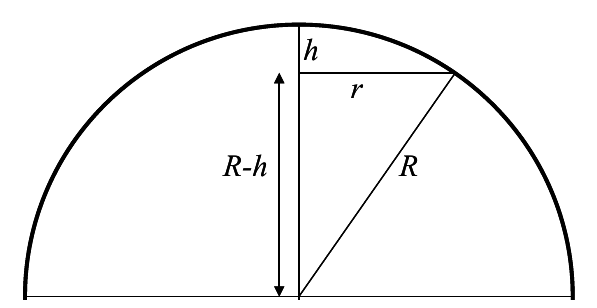
\includegraphics[width=\textwidth]{Krivinski_polmer}
\end{figure}
S pomočjo pravokotnega trikotni lahko izpeljemo sledečo formulo:


\begin{equation}
  \begin{gathered}
    R^2 = (R - h)^2 + r^2 \\
    R^2 = R^2 - 2Rh + h^2 + r^2 \\
    R = \frac{h^2 + r^2}{2h}
  \end{gathered}
\end{equation}

Če v formulo vstavimo podatke dobimo:

\begin{equation}
  \begin{gathered}
    R = \frac{4.29^2 \cdot (1 \ \pm \ 2 \cdot 0.002) \ mm^2 + 29.9^2 \cdot (1 \ \pm \ 2 \cdot 0.007) \ mm^2}{2 \cdot 4.29 \cdot (1 \ \pm \ 0.002) \ mm}\\
    R = \frac{(18.4 \ \pm \ 0.01) \ mm^2 + (894 \ \pm \ 13) \ mm^2}{8.58 \cdot (1 \ \pm \ 0.002) \ mm}\\
    R = \frac{(912 \ \pm \ 13) \ mm^2}{8.58 \cdot (1 \ \pm \ 0.002) \ mm}\\
    R = \frac{912 \cdot (1 \ \pm \ 0.01) \ mm}{8.58 \cdot (1 \ \pm \ 0.002)}\\
    \boxed{R = 106 \cdot (1 \ \pm \ 0.01) \ mm}
  \end{gathered}
\end{equation}



\pagebreak
\section{Mikroskop}
\subsection{Navodila}
\bm{a)} Umerite merilno mrežo mikroskopa in izmerite premer tanke žičke, premer majhne
luknjice, debelino svojega lasu in število nitk na milimeter pri mrežici za sitotisk.\\\\
\bm{b)}  Z navadnim ravnilom skušajte na \bm{0.1 \ mm} natančno izmeriti debelino črte, ki
je tanjša od \bm{1 \ mm}. Ocenite napako take meritve. Nato debelino črte izmerite še z merilnim
mikroskopom in preverite, ali ste z ravnilom debelino pravilno ocenili.

\pagebreak
\subsection{Meritve}

Meritve sem opravil na štirih različnih predmetih, in sicer: na lasu, 
žici, luknjici in na črti.\\\\
Merilo:
$10.1 \ enot \ldots 1 \ mm$

\begin{table}[H]
  \centering
  \caption{Premer lasu}
  \begin{adjustwidth}{-1.5cm}{0cm}
  \begin{tabular}{cccccccccc}
  \midrule
  Meritev & $l_{izm} \ [enot]$ & $\overline{h} \ [enot]$ & $h_{izm} - \overline{h} \ [enot]$ & $\sigma \ [enot]$ & $\Delta h_{sl} \ [enot]$ & $\Delta h_{sist} \ [enot]$ & $h \ [enot]$\\
  \midrule
  1 & 0.7 & \multirow{10}{*}{0.8} & \sout{-0.1} & \multirow{10}{*}{0} & \multirow{10}{*}{0} & \multirow{10}{*}{0.1} & \multirow{4}{*}{0.8 \ \pm \ 0.1}\\
  2 & 0.8 & & 0\\
  3 & 0.8 & & 0\\
  4 & 0.7 & & \sout{-0.1}\\
  5 & 0.7 & & \sout{-0.1} & & & & \multirow{2}{*}{=}\\
  6 & 0.8 & & 0 \\
  7 & 0.8 & & 0 & & & & \multirow{4}{*}{$0.8 \cdot (1 \ \pm \ 0.1)$}\\
  8 & 0.8 & & 0\\
  9 & 0.8 & & 0\\
  10 & 0.8 & & 0\\
  % Add more rows here
  \midrule
  \end{tabular}
\end{adjustwidth}
\end{table}

\begin{centering}
  Premer lasu: $0.08 \cdot (1 \ \pm 0.1) \ mm$
\end{centering}


\begin{table}[H]
  \centering
  \caption{Premer žice}
  \begin{adjustwidth}{-1.5cm}{0cm}
  \begin{tabular}{cccccccccc}
  \midrule
  Meritev & $z_{izm} \ [enot]$ & $\overline{z} \ [enot]$ & $z_{izm} - \overline{z} \ [enot]$ & $\sigma \ [enot]$ & $\Delta z_{sl} \ [enot]$ & $\Delta z_{sist} \ [enot]$ & $z \ [enot]$\\
  \midrule
  1 & 3.1 & \multirow{10}{*}{3.2} & \sout{-0.1} & \multirow{10}{*}{0.1} & \multirow{10}{*}{0} & \multirow{10}{*}{0.1} & \multirow{4}{*}{3.2 \ \pm \ 0.1}\\
  2 & 3.2 & & 0\\
  3 & 3.1 & & \sout{-0.1}\\
  4 & 3.2 & & 0\\
  5 & 3.2 & & 0 & & & & \multirow{2}{*}{=}\\
  6 & 3.2 & & 0 \\
  7 & 3.1 & & \sout{-0.1} & & & & \multirow{4}{*}{$3.2 \cdot (1 \ \pm \ 0.03)$}\\
  8 & 3.1 & & -0.1\\
  9 & 3.1 & & -0.1\\
  10 & 3.2 & & 0\\
  % Add more rows here
  \midrule
  \end{tabular}
\end{adjustwidth}
\end{table}

\begin{centering}
  Premer žice: $0.32 \cdot (1 \ \pm 0.03) \ mm$
\end{centering}

\begin{table}[H]
  \centering
  \caption{Premer luknjice}
  \begin{adjustwidth}{-1.5cm}{0cm}
  \begin{tabular}{cccccccccc}
  \midrule
  Meritev & $l_{izm} \ [enot]$ & $\overline{l} \ [enot]$ & $l_{izm} - \overline{l} \ [enot]$ & $\sigma \ [enot]$ & $\Delta l_{sl} \ [enot]$ & $\Delta l_{sist} \ [enot]$ & $l \ [enot]$\\
  \midrule
  1 & 7.2 & \multirow{10}{*}{7.2} & 0 & \multirow{10}{*}{0.1} & \multirow{10}{*}{0} & \multirow{10}{*}{0.1} & \multirow{4}{*}{7.2 \ \pm \ 0.1}\\
  2 & 7.8 & & \sout{0.6}\\
  3 & 7.1 & & \sout{-0.1}\\
  4 & 7.2 & & 0\\
  5 & 7.2 & & 0 & & & & \multirow{2}{*}{=}\\
  6 & 7.1 & & \sout{-0.1} \\
  7 & 7.3 & & 0.1 & & & & \multirow{4}{*}{$7.2 \cdot (1 \ \pm \ 0.01)$}\\
  8 & 7.1 & & -0.1\\
  9 & 7.2 & & 0\\
  10 & 7.1 & & -0.1\\
  % Add more rows here
  \midrule
  \end{tabular}
\end{adjustwidth}
\end{table}

\begin{centering}
  Premer luknjice: $0.71 \cdot (1 \ \pm 0.01) \ mm$
\end{centering}


\begin{table}[H]
  \centering
  \caption{Širina črte}
  \begin{adjustwidth}{-1.5cm}{0cm}
  \begin{tabular}{cccccccccc}
  \midrule
  Meritev & $b_{izm} \ [enot]$ & $\overline{b} \ [enot]$ & $b_{izm} - \overline{b} \ [enot]$ & $\sigma \ [enot]$ & $\Delta b_{sl} \ [enot]$ & $\Delta b_{sist} \ [enot]$ & $b \ [enot]$\\
  \midrule
  1 & 5.0 & \multirow{10}{*}{5.4} & \sout{-0.4} & \multirow{10}{*}{0.1} & \multirow{10}{*}{0} & \multirow{10}{*}{0.1} & \multirow{4}{*}{5.4 \ \pm \ 0.1}\\
  2 & 5.4 & & 0\\
  3 & 5.5 & & 0.1\\
  4 & 5.4 & & 0\\
  5 & 5.5 & & \sout{0.1} & & & & \multirow{2}{*}{=}\\
  6 & 5.4 & & 0 \\
  7 & 5.3 & & -0.1 & & & & \multirow{4}{*}{$5.4 \cdot (1 \ \pm \ 0.02)$}\\
  8 & 5.2 & & \sout{-0.2}\\
  9 & 5.3 & & -0.1\\
  10 & 5.5 & & 0.1\\
  % Add more rows here
  \midrule
  \end{tabular}
\end{adjustwidth}
\end{table}

\begin{centering}
  Širina črte: $0.53 \cdot (1 \ \pm 0.02) \ mm$
\end{centering}

%%%%%%%%%%% Laser %%%%%%%%%%%



\pagebreak
\section{Meritve z lasersko svetlobo}

\begin{figure}[H]
  \caption{Slika za prvi uklon}
  \label{fig:graf}
  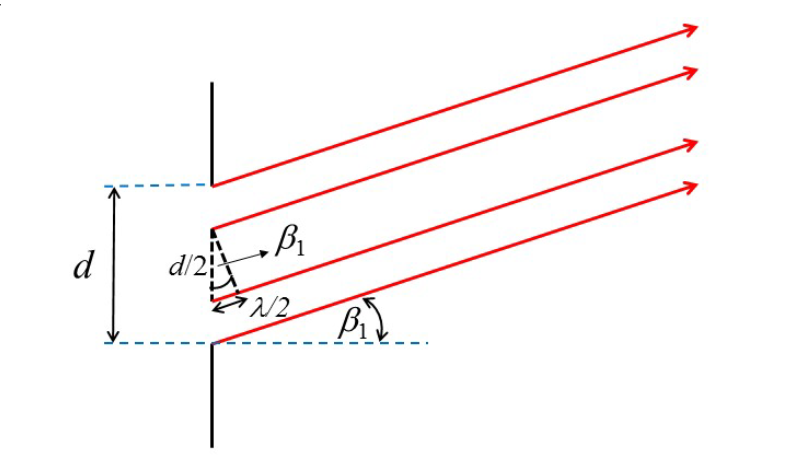
\includegraphics[width=\textwidth]{uklonska_mrezica}
\end{figure}

Za N-to oslabitev velja:\\
\begin{equation}
  d \sin{\beta_{N} = N \lambda}  
\end{equation}\\
Če uporabimo približek za male kote, da je $ \sin{\beta} \approx \beta$.
\\\\
Tako dobimo enačbo:
\begin{equation}
  d \beta_{N} = N \lambda  
\end{equation}

\noindent Pravtako pa lahko do kota \beta \ pridemo preko razmerja med oslabitvijo in
razdalijo do zaslona.\\
\begin{equation}
  \tan{\beta_{N}} = \frac{x_N}{L}  
\end{equation}
Uporabimo približek za male kote, da je $ \tan{\beta} \approx \sin{\beta} \approx \beta$.\\
\begin{equation}
  \beta_{N} = \frac{x_N}{L}  
\end{equation}\\\\
Z združitvijo enačbe 3.9 in 3.11 dobimo enačbo širine reže uklonske mrežice.
\begin{equation}
  d = \frac{N \lambda L}{x_{N}}
\end{equation}

\noindent Napaka ravnila: $\bm{0.1 \ cm}$\\
Valovna dolžina laserja: $\lambda = \bm{532 \ nm}$\\
Dolžina od zaslona: $L = \bm{257 cm}$

\begin{table}[H]
  \centering
  \caption{Meritve oslabitev levo}
  \begin{tabular}{cccccccccc}
  \toprule
  Oslabitev levo & $x_{N \ izm} \ [cm]$ & $\frac{x_{N \ izm}}{N} \ [cm]$\\
  \midrule
  1 & 0.9 & 0.9\\
  2 & 1.9 & 0.95\\
  3 & 2.8 & 0.93\\
  4 & 3.8 & 0.95\\
  5 & 4.7 & 0.94\\
  6 & 5.6 & 0.93\\
  7 & 6.6 & 0.94\\
  % Add more rows here
  \bottomrule
  \end{tabular}
\end{table}

\begin{table}[H]
  \centering
  \caption{Meritve oslabitev desno}
  \begin{tabular}{cccccccccc}
  \toprule
  Oslabitev levo & $x_{N \ izm} \ [cm]$ & $\frac{x_{N \ izm}}{N} \ [cm]$\\
  \midrule

  1 & 1.0 & 1.0\\
  2 & 2.0 & 1.0\\
  3 & 2.9 & 0.97\\
  4 & 3.9 & 0.98\\
  5 & 4.9 & 0.98\\
  6 & 5.9 & 0.98\\
  7 & 6.9 & 0.99\\
  % Add more rows here
  \bottomrule
  \end{tabular}
\end{table}

\begin{table}[H]
  \centering
  \caption{Zbrane meritve}
  \begin{tabular}{cccccccccc}
  \toprule
  Meritev & $\frac{x_{N \ izm}}{N} \ [cm]$ & $\overline{\frac{x_{N \ izm}}{N}} \ [cm]$ & $\frac{x_{N \ izm}}{N} \ [cm]$ - $\overline{\frac{x_{N \ izm}}{N}} \ [cm]$ & $\frac{x_{N}}{N} \ [cm]$\\
  \midrule
  1 & 0.9 & \multirow{14}{*}{1.0} & \sout{0.1} & \multirow{6}{*}{1.0 \ \pm \ 0.1}\\
  2 & 0.95 & & 0 &\\
  3 & 0.93 & & \sout{0.1} &\\
  4 & 0.95 & & 0 &\\
  5 & 0.94 & & \sout{0.1} &\\
  6 & 0.93 & & \sout{0.1} &\\
  7 & 0.94 & & \sout{0.1} & \multirow{2}{*}{=}\\
  8 & 1.0 & & 0 &\\
  9 & 1.0 & & 0 & \multirow{6}{*}{1.0 \cdot \ (1\ \pm \ 0.1)}\\
  10 & 0.97 & & 0 &\\
  11 & 0.98 & & 0 &\\
  12 & 0.98 & & 0 &\\
  13 & 0.98 & & 0 &\\
  14 & 0.99 & & 0 &\\
  % Add more rows here
  \bottomrule
  \end{tabular}
\end{table}

\pagebreak
\subsubsection{Izračuni širine reže uklonske mrežice}

\begin{equation}
  \label{eq:1}
  \begin{gathered}
    d = \left( \frac{x_{N}}{N} \right)^{-1} \lambda L \\
    d = (1.0 \cdot 10^{-2} \cdot (1\ \pm \ 0.1) \ m)^{-1} \cdot 532 \cdot 10^{-9} \ m \cdot 257 \cdot 10^{-2} \ m\\
    d = 1.0 \cdot 10^{2} \cdot (1\ \pm \ 0.1) \ m^{-1} \cdot 532 \cdot 10^{-9} \ m \cdot 257 \cdot 10^{-2} \ m\\
    \boxed{
      d = 1.4 \cdot 10^{-4} \ m
    }
  \end{gathered}
\end{equation}
\pagebreak

\section{Vprašanja}
Katere pomembne lastnosti ima laserska svetloba, da lahko z njo opravljamo interferenčne
poskuse? Ali bi poskus uspel s sončno svetlobo? Pri odgovoru na vprašanje si pomagajte
z literaturo.\\\\

\noindent Laserska svetloba ima več pomembnih lastnosti, ki omogočajo izvajanje interferenčnih poskusov:

\begin{enumerate}
    \item \textbf{Koharenca:} Laserska svetloba je kohernetna, kar pomeni, da ima dolg koherenčni čas. To je čas, v katerem lahko ohranja stabilno fazo. To je ključno za interferenco, saj se interferenčni vzorci oblikujejo na podlagi faznih razlik med valovi.
    
    \item \textbf{Monokromatičnost:} Laserska svetloba je monokromatska, kar pomeni, da ima ožji spekter valovnih dolžin. To omogoča enakomerno interferenco, saj so valovi med seboj povezani na podlagi svojih valovnih dolžin.
    
    \item \textbf{Usmerjenost:} Laserski snop je običajno zelo usmerjen, kar pomeni, da se svetloba širi v relativno ozkem snopu. To je pomembno za natančne interferenčne poskuse.
    
    \item \textbf{Visoka svetlobna gostota:} Laserska svetloba ima visoko svetlobno gostoto, kar omogoča intenzivne interferenčne vzorce.
\end{enumerate}
Glede na te lastnosti bi interferenčni poskusi s sončno svetlobo bili manj uspešni. Sončna svetloba ni koherentna na enak način kot laserska svetloba, saj je sestavljena iz več valovnih dolžin in ni usmerjena. Interferenčni vzorci, pridobljeni s sončno svetlobo, bi bili običajno manj izraziti in manj stabilni.\\
Za izvedbo natančnih interferenčnih poskusov je torej priporočljivo uporabljati lasersko svetlobo zaradi njenih zgoraj omenjenih lastnosti.



\chapter{Vaja 4: Merjenje frekvence}

\section{Naloga}
Izmerite frekvenco vrtenja plošče, ki je pritrjena na elektromotor na dva načina:\\\\
\textbf{a)} z elektronskim merilnikom frekvence,\\
\textbf{b)} z modelom merilnika frekvence.\\\\
Primerjajte rezultata obeh meritev pri različnih frekvencah vrtenja plošče.\\\\
Te meritve sem opravil pri napetostih: \textbf{5 V, 6 V, 7 V, 9 V} in \textbf{12 V}, za vsako napetost 5-krat.
\afterpage{
\section{Meritve}

Najprej sem opravil meritve s pomočjo elektronskega merilnika frekvence.

\begin{table}[H]

\caption{Merjenje frekvence uporabo elektronskega merilnika frekvence}
\begin{adjustwidth}{-3.5 cm}{0 cm}
\begin{tabular}{cccccccccccc}
\toprule
Meritev & Napetost & $\nu_{izm}$~[min\textsuperscript{-1}] & $\overline\nu$ & $\nu_{izm}$ - $\overline\nu$~[min\textsuperscript{-1}] &$\Delta\nu_{sist}$~[min\textsuperscript{-1}] & \sigma &$\Delta\nu_{slu}$ [min\textsuperscript{-1}] & \nu~[Hz]\\

%pri 5V

\midrule
1 & \multirow{5}{*}{5.0 V} & 654.4 & \multirow{5}{*}{658.9} & -4.5 & \multirow{5}{*}{0.1} & \multirow{5}{*}{6.5} & \multirow{5}{*}{2.9} & \\
2 & & 670.5 & & \sout{11.6}  & & & & $10.98 \ \pm \ 0.05$\\
3 & & 665.3 & & 6.4 & & & & =\\
4 & & 657.0 & & -1.9 & & & & $ 10.98 \cdot (1 \ \pm \ 0.005) $\\
5 & & 647.4 & & \sout{-11.5} &\\

%pri 6V

\midrule
6 & \multirow{5}{*}{6.0 V} & 1058 &  \multirow{5}{*}{1053} & 5 & \multirow{5}{*}{1} & \multirow{5}{*}{6} & \multirow{5}{*}{3} & \\
7 & & 1054 & & 1 & & & & $17.55 \ \pm \ 0.07$\\
8 & & 1037 & & \sout{-16} & & & & =\\
9 & & 1053 & & 0 & & & & $17.55 \cdot (1 \ \pm \ 0.004)$\\
10 & & 1062 & & \sout{9} & \\

%pri 7V

\midrule
11 & \multirow{5}{*}{7.0 V} & 1576 & \multirow{5}{*}{1563} & \sout{13} & \multirow{5}{*}{1} & \multirow{5}{*}{13}  & \multirow{5}{*}{6} & \\
12 & & 1575 & & 12 & & & & $ 26.1 \ \pm \ 0.1 $\\
13 & & 1532 & & \sout{-31} & & & & =\\
14 & & 1567 & & 4 & & & & $26.1 \cdot (1 \ \pm \ 0.004)$\\
15 & & 1565 & & 2 &\\

%pri 9 V

\midrule
16 & \multirow{5}{*}{9.0 V} & 2351 & \multirow{5}{*}{2413} & \sout{-62} & \multirow{5}{*}{1} & \multirow{5}{*}{57} & \multirow{5}{*}{25} & \\
17 & & 2354 & & \sout{-59} & & & & $ 40.2 \ \pm \ 0.2 $\\
18 & & 2449 & & 36 & & & & =\\
19 & & 2469 & & 56 & & & & $40.2 \cdot (1 \ \pm \ 0.005)  $\\
20 & & 2444 & & 31 &\\

%pri 12 V

\midrule
21 & \multirow{5}{*}{12.0 V} & 3917 & \multirow{5}{*}{3937} & -20 & \multirow{5}{*}{1} & \multirow{5}{*}{27} & \multirow{5}{*}{12} & \\
22 & & 3972 & & \sout{35} & & & & $65.6 \ \pm \ 0.5$\\
23 & & 3963 & & 26 & & & & =\\
24 & & 3905 & & \sout{-32} & & & & $65.6 \cdot (1 \ \pm \ 0.008) $\\
25 & & 3926 & & -11\\
% Add more rows here
\bottomrule
\end{tabular}
\end{adjustwidth}
\end{table}
}
\pagebreak





%% druga tabela %%%%

Nato sem za merjenje nihajnjega časa uporabil osciloskop.

\begin{table}[H]

\caption{Mejrenje frekvence z uporabo osciloskopa}
\begin{adjustwidth}{-2.5 cm}{0 cm}
\begin{tabular}{cccccccccccc}
\toprule
Meritev & Napetost & $t_{izm} [s]$ & $\overline{t} \ [s]$ & $t_{izm}$ - $\overline{t} \ [s]$ & $t_{sist} \ [s]$ & \sigma & $\Delta t_{slu} [s]$ & \nu~[Hz]\\

%pri 5V

\midrule
1 & \multirow{5}{*}{5.0 V} & -0.080 & \multirow{5}{*}{0.088} & \sout{-0.008} & \multirow{5}{*}{0.004} & \multirow{5}{*}{0} & \multirow{5}{*}{0} & \\
2 & & 0.096 & & \sout{0.008}  & & & & $11 \cdot (1\ \pm \ 0.05)$\\
3 & & 0.088 & & 0 & & & & = \\
4 & & 0.088 & & 0 & & & & $11 \ \pm \ 1$\\
5 & & 0.088 & & 0 &\\

%pri 6V

\midrule
6 & \multirow{5}{*}{6.0 V} & 0.052 &  \multirow{5}{*}{0.052} & 0 & \multirow{5}{*}{0.002} & \multirow{5}{*}{0} & \multirow{5}{*}{0} &\\
7 & & 0.052 & & 0 & & & & $19 \cdot (1\ \pm \ 0.05)$\\
8 & & 0.050 & & \sout{-0.02} & & & & =\\
9 & & 0.052 & & 0 & & & & $19 \ \pm \ 1 $\\
10 & & 0.052 & & \sout{0} & \\

%pri 7V

\midrule
11 & \multirow{5}{*}{7.0 V} & 0.036 & \multirow{5}{*}{0.038} & \sout{-0.002} & \multirow{5}{*}{0.001} & \multirow{5}{*}{0} & \multirow{5}{*}{0} & \\
12 & & 0.038 & & 0 & & & & $26 \cdot (1 \ \pm \ 0.03) $\\
13 & & 0.038 & & 0 & & & & =\\
14 & & 0.039 & & \sout{0.001} & & & & $26 \ \pm \ 1$\\
15 & & 0.038 & & 0 &\\

%pri 9 V

\midrule
16 & \multirow{5}{*}{9.0 V} & 0.024 & \multirow{5}{*}{0.023} & \sout{0.001} & \multirow{5}{*}{0.001} & \multirow{5}{*}{0} & \multirow{5}{*}{0}\\
17 & & 0.023 & & 0 & & & & $43 \cdot (1 \ \pm \ 0.04)$\\
18 & & 0.022 & & \sout{-0.001} & & & & =\\
19 & & 0.023 & & 0 & & & & $43 \ \pm \ 2$\\
20 & & 0.023 & & 0 &\\

%pri 12 V

\midrule
21 & \multirow{5}{*}{12.0 V} & 0.0152 & \multirow{5}{*}{0.0150} & 0.0002 & \multirow{5}{*}{0.0004} & \multirow{5}{*}{0.0002} & \multirow{5}{*}{0.0001}\\
22 & & 0.0152 & & \sout{0.0002} & & & & $66.7 \cdot (1 \ \pm \ 0.03)$\\
23 & & 0.0148 & & -0.0002 & & & & =\\
24 & & 0.0148 & & \sout{-0.0002} & & & & $66.7 \ \pm \ 2.0 $\\
25 & & 0.0148 & & -0.0002\\
% Add more rows here
\bottomrule
\end{tabular}
\end{adjustwidth}
\end{table}
  
\pagebreak
\section{Rezultati}
Pri rezultatih lahko opazimo, da so meritve, pri čemer smo merili frekvenco in ne čas, 
bolj natančne. To je zato, ker je čas nihanja obratna vrednost hitrosti in že pri zelo mali spremembi
časa lahko pride do velike spremembe frekvence. Medtem, ko smo pri merjenju z uporabo merilnika hitrosti
merili frekvenco samo in do tega ni moglo priti.


\section{Vprašanja}

\textbf{a)} Kvalitativno razložite fizikalno delovanje diode in fotodiode
(podrobnejšo razlago boste slišali pri moderni fiziki in pri predmetih s področja fizike trdne snovi, 
fizike materialov in statistični termodinamiki v višjih letnikih).

\smallskip

\noindent Dioda je polprevodniški elektronski element. To pomeni, da v eni smeri električni tok prepušča, v drugi pa ne.
Za to je uporabna pri usmerjanju izmeničnih siginalov.
Fotodioda pa je dioda, ki deluje na principu fotoelektričnega pojava. Ob večji svetlobi po fotodiodi teče močnejši tok,
pri nižji pa šibkejši.

\bigskip


\noindent \textbf{b)} Kvalitativno razložite delovanje osciloskopa, 
ki temelji na principu katodne cevi (CRT): 
kako v katodni cevi ustvarimo proste elektrone, kako jih pospešimo, 
kako jih uklanjamo v vodoravni in navpični smeri.

\smallskip

\noindent Osciloskop je elektronska merilna naprava, ki omogoča opazovanje napetosti.
Ponavadi jih uporabljamo za opazovvanje oblike električnega siginala ter njegove amplitude.
Zaslon osciloskopa temelji na principu katodne cevi. V katodni cevi so katodni žarki; 
to so hitri tokovi elektronov, ki izhajajo iz ogrete katode v vakuumski cevi. V cevi so elektroni usmerjeni v žarek, ki potuje proti anodi na vidnem koncu. Ta anoda je prekrita z luminiscenčnim materialom, ki odda svetlobo, ko nanjo trčijo elektroni. To se doseže z uporabo magnetnega ali električnega polja, ki usmerja elektrone in povzroča svetlobno emisijo ob trku z anodo.

\end{document}
